\documentclass[mathserif,hyperref={urlcolor=cyan,colorlinks=true}]{beamer}
\usepackage[utf8]{inputenc}

\usetheme{Warsaw}
%\usetheme{Ilmenau}
%\usetheme{Berlin}

%\usecolortheme{orchid}
%\usecolortheme{rose}
%\usecolortheme{whale}

\usepackage{lmodern}
\usepackage[T1]{fontenc}
\usepackage{textcomp}

\beamertemplatenavigationsymbolsempty
\setbeamertemplate{footline}{}

\title{Non-canonical XS Objects\\With a Bit of Perl Magic}
\author{Sergey Aleynikov}
\institute{Crazy Panda}
\date[May 2015]{YAPC Russia 2015}
\begin{document}

\begin{frame}
\titlepage
\end{frame}

{
%\setbeamercolor{background canvas}{bg=black}
%\setbeamertemplate{frametitle}[default][colsep=-4bp,rounded=false,shadow=false]
\begin{frame}{Canonical XS objects}
\only<0>{
\begin{block}{DateTIme.xs}
SV*\newline\noindent
DateTime::new()\newline\noindent
CODE:\newline\noindent
\phantom{x}\hspace{1em}DateTime* THIS = new DateTime();\newline\noindent
\newline\noindent
\phantom{x}\hspace{1em}RETVAL = newSV(0);\newline\noindent
\phantom{x}\hspace{1em}SV* intref = newSVrv(RETVAL, CLASS);\newline\noindent
\phantom{x}\hspace{1em}sv{\_}setiv(intref, PTR2IV(THIS));\newline\noindent
OUTPUT:\newline\noindent
\phantom{x}\hspace{1em}RETVAL
\end{block}
}

\begin{figure}
\scalebox{0.65}{
    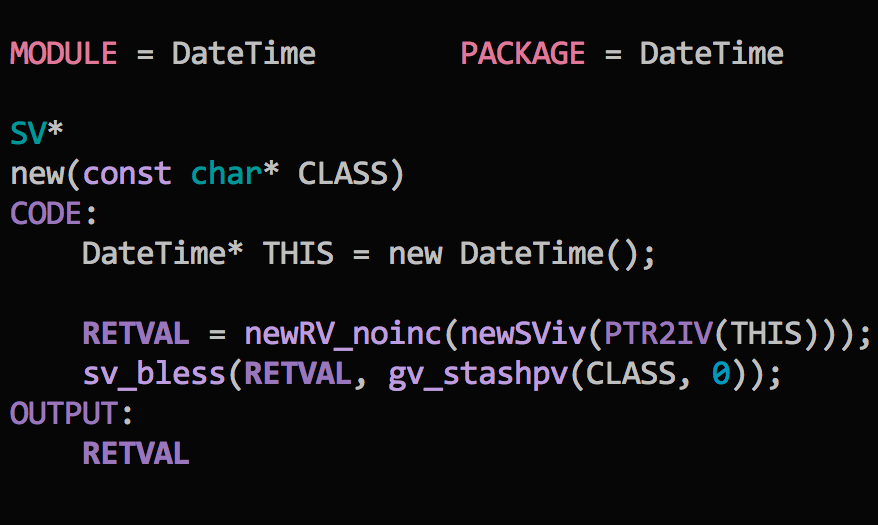
\includegraphics{new_nont.png}
}
\end{figure}

\end{frame}
}

\begin{frame}{Accessing canonical object}
\only<0>{
\begin{block}{DateTIme.xs}
void\newline\noindent
DateTime::dump(SV* obj)\newline\noindent
CODE:\newline\noindent
\phantom{x}\hspace{1em}if (!sv{\_}isobject(obj))\newline\noindent
\phantom{x}\hspace{3em}croak("Not a DateTime object");\newline\noindent
\phantom{x}\hspace{1em}DateTime* THIS = (DateTime*)SvIV(SvRV(obj));\newline\noindent
\phantom{x}\hspace{1em}THIS->dump();\newline\noindent
\end{block}
}

\begin{figure}
\scalebox{0.65}{
    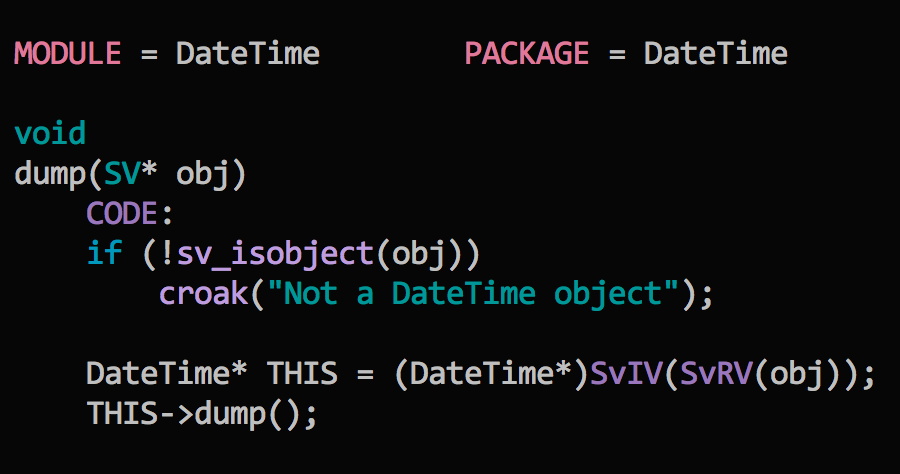
\includegraphics{dump-nont.png}
}
\end{figure}

\end{frame}

\begin{frame}{Typemaps - write less}
\begin{block}{typemap}
DateTime*\hspace{1em}O{\_}OBJECT
\end{block}
%\pause

\only<0>{
\begin{block}{DateTIme.xs}
DateTIme*\newline\noindent
DateTIme::new()\newline\noindent
CODE:\newline\noindent
\phantom{x}\hspace{1em}RETVAL = new DateTime();\newline\noindent
OUTPUT:\newline\noindent
\phantom{x}\hspace{1em}RETVAL\newline\noindent
\newline\noindent
void\newline\noindent
DateTime::dump()\newline\noindent
CODE:\newline\noindent
\phantom{x}\hspace{1em}THIS->dump();\newline\noindent
\end{block}
}

\begin{figure}
\scalebox{0.6}{
    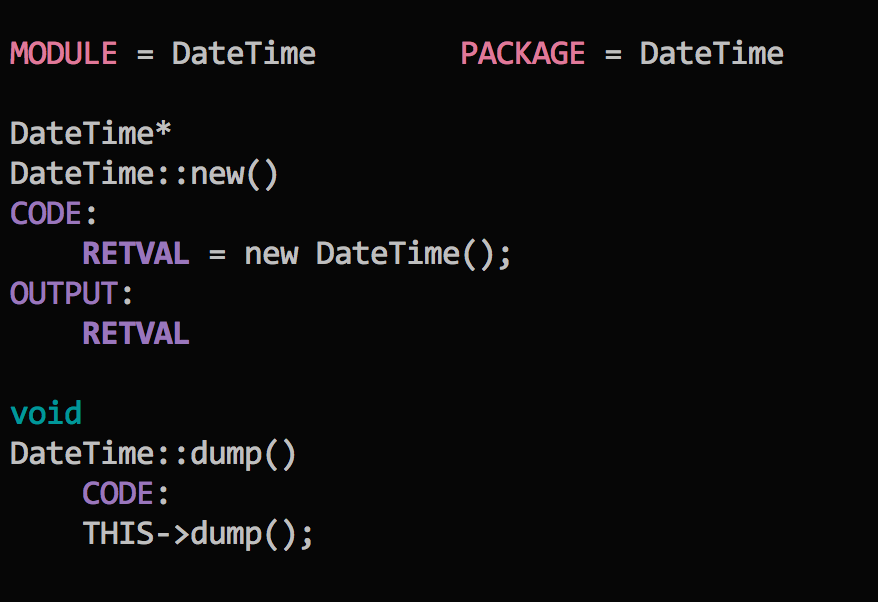
\includegraphics{new-tmap.png}
}
\end{figure}

\end{frame}

\begin{frame}{Why not?}
    \begin{columns}[c]
    \column{.5\textwidth}
        \begin{exampleblock}{Pros}
        \begin{itemize}
            \item Straightforward
            \item Inside a default typemap
            \item Fast unpack
        \end{itemize}
        \end{exampleblock}
    \column{.5\textwidth}
        \uncover<2->{
        \begin{alertblock}{Cons}
        \begin{itemize}
            \item No additional data
            \item One C object per Perl object
            \item Visible at Perl level
        \end{itemize}
        \end{alertblock}
        }
    \end{columns}
\end{frame}

\begin{frame}[fragile]{What is Perl magic?}
\begin{figure}
    \scalebox{0.35}{
        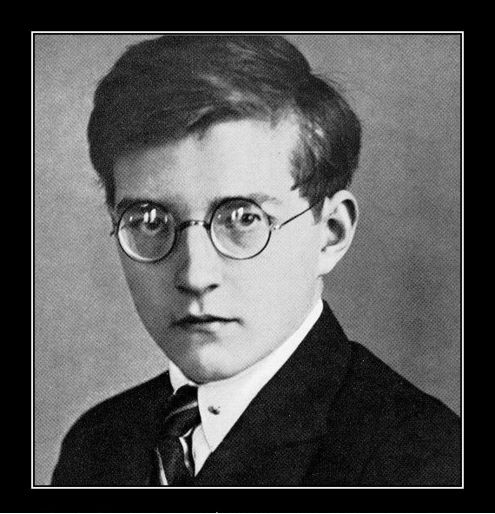
\includegraphics{Shostakovich.jpg}
    }
%\pause
\begin{center}
{\bf
{\tiny
    \begin{verbatim}
    perl -e '$??s:;s:s;;$?::s;;=]=>%-{<-|}<&|`{;;y; -/:-@[-`{-};`-{/" -;;s;;$_;see'
    \end{verbatim}
}
}
\end{center}
\end{figure}
\end{frame}

\begin{frame}{What is Perl magic indeed?}
\begin{figure}
\scalebox{0.35}{
    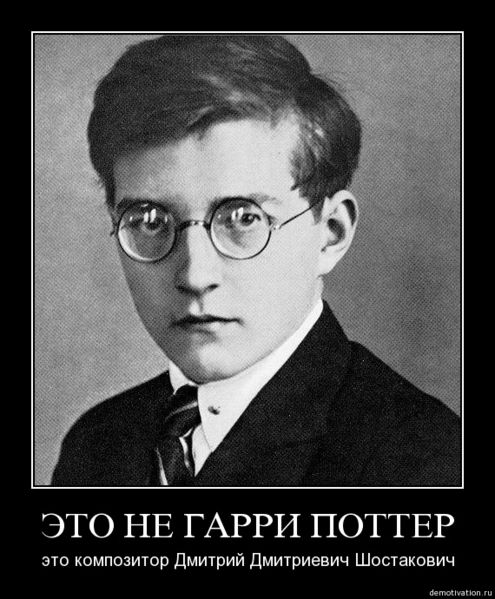
\includegraphics{Shostakovich_unv.jpg}
}
\end{figure}
\end{frame}

\begin{frame}{True magic}
\begin{itemize}
\item<1-> @ISA
\item<1-> \%\^{}H
\item<1-> \%SIG
\item<1-> \$!
\item<1-> \$DB::single
\item<2-> referee behind weaken()'d reference
\item<3-> tie()'d variable
\item<4-> more than 40 types of built-in magic
\end{itemize}
\end{frame}

\begin{frame}{How it works?}
\begin{itemize}
\item<1-> Acts on event trigger
    \begin{itemize}
    \item<2-> svt{\_}get
    \item<2-> svt{\_}set
    \item<2-> svt{\_}free
    \item<2-> svt{\_}clear
    \end{itemize}
\item<3-> Special types are checked at various places
\item<4-> PERL{\_}MAGIC{\_}ext reserved for extensions
\item<5-> sv{\_}magicext API call
\end{itemize}
\end{frame}

\begin{frame}{Creating magical object}
\only<0>{
\begin{block}{DateTime.xs}
STATIC MGVTBL marker;\newline\noindent
\newline\noindent
SV*\newline\noindent
DateTime::new()\newline\noindent
CODE:\newline\noindent
\phantom{x}\hspace{1em}RETVAL = newRV{\_}noinc(\&PL{\_}sv{\_}undef);\newline\noindent
\phantom{x}\hspace{1em}sv{\_}bless(RETVAL, gv{\_}stashpv(CLASS, 0));\newline\noindent
\phantom{x}\hspace{1em}DateTime* THIS = new DateTime();\newline\noindent
\phantom{x}\hspace{1em}sv{\_}magicext(RETVAL, NULL, PERL{\_}MAGIC{\_}ext, \&marker, (const char*)THIS, 0);\newline\noindent
\phantom{x}\hspace{1em}SvRMAGICAL{\_}off(RETVAL);\newline\noindent
OUTPUT:\newline\noindent
\phantom{x}\hspace{1em}RETVAL\newline\noindent
\end{block}
}

\begin{figure}
\scalebox{0.6}{
    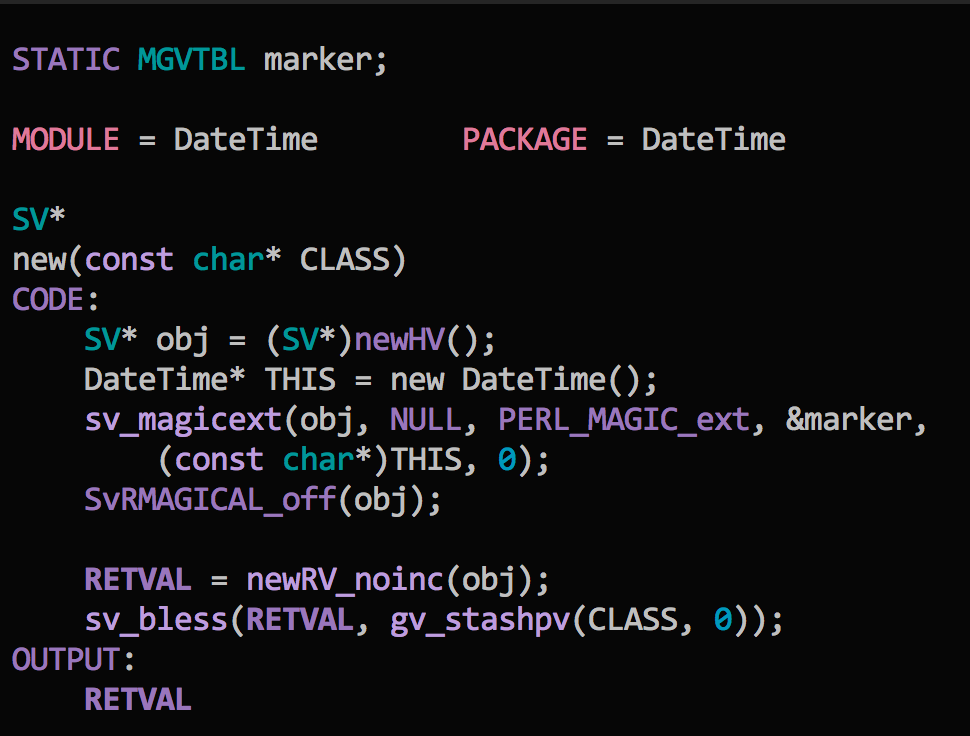
\includegraphics{new-magic.png}
}
\end{figure}

\end{frame}

\begin{frame}{Accessing magical object}
\only<0>{
\begin{block}{DateTime.xs}
void\newline\noindent
DateTime::dump()\newline\noindent
CODE:\newline\noindent
\phantom{x}\hspace{1em}MAGIC* mg = mg{\_}findext(THIS, PERL{\_}MAGIC{\_}ext, \&marker);\newline\noindent
\phantom{x}\hspace{1em}if (!mg) croak("Not a DateTime object");\newline\noindent
\phantom{x}\hspace{1em}DateTime* THIS = (DateTime*)mg->mg{\_}ptr;\newline\noindent
\phantom{x}\hspace{1em}THIS->dump();\newline\noindent
\end{block}
}

\begin{figure}
\scalebox{0.5}{
    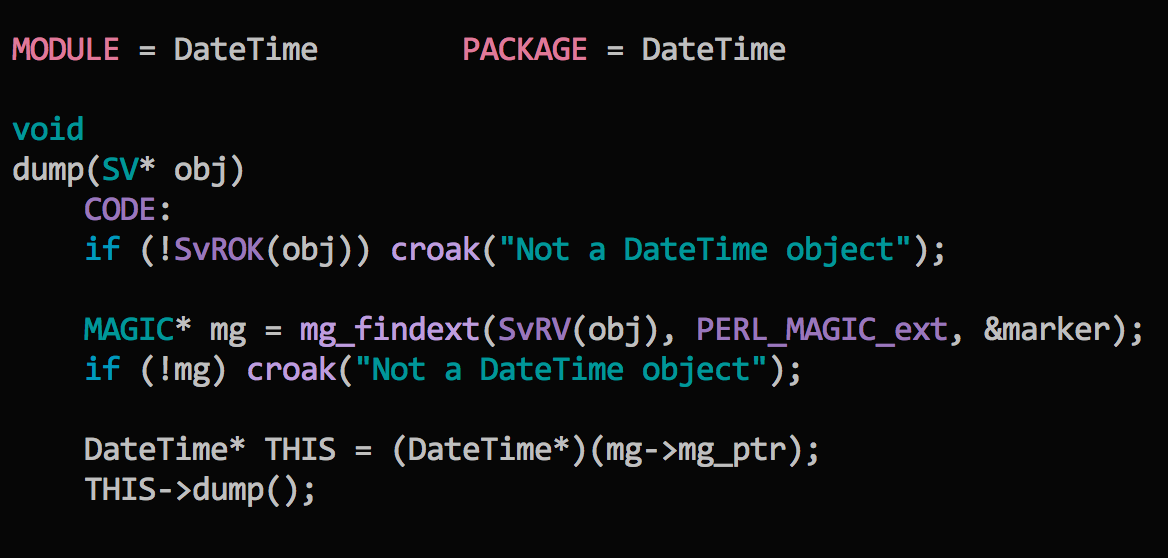
\includegraphics{dump-magic.png}
}
\end{figure}

\end{frame}

\begin{frame}{Lifecycle}
\begin{figure}
\scalebox{0.5}{
    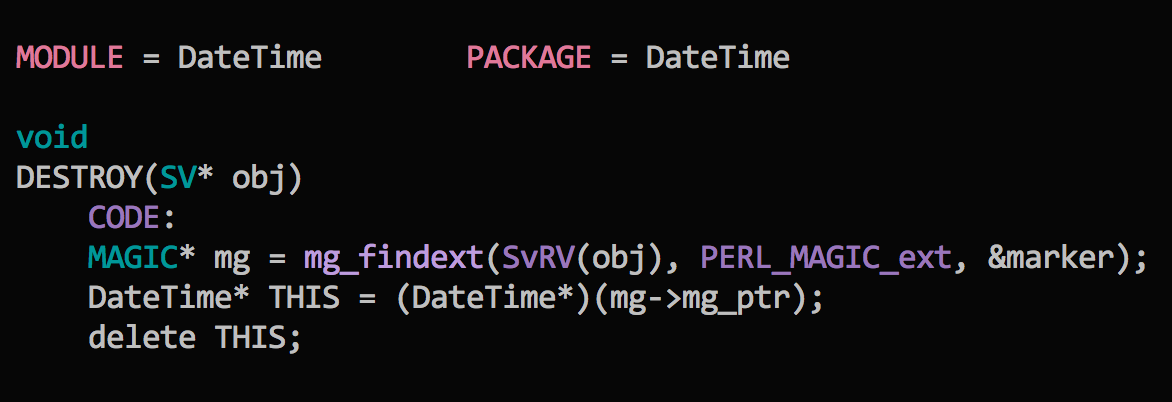
\includegraphics{destroy-magic.png}
}
\end{figure}
\end{frame}

\begin{frame}{Example}
\begin{figure}
\scalebox{0.7}{
    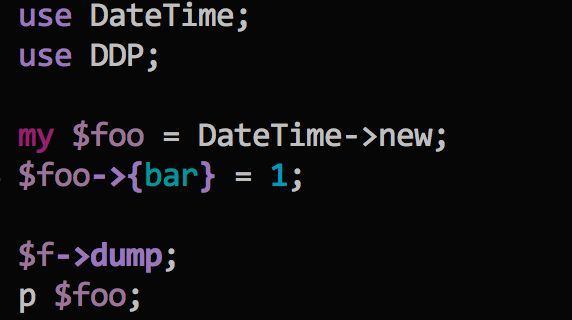
\includegraphics{ex-1.png}
}
\end{figure}
\begin{figure}
\scalebox{0.7}{
    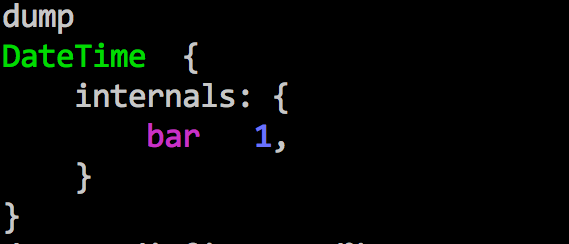
\includegraphics{ex-2.png}
}
\end{figure}
\end{frame}

\begin{frame}{Extending objects}
\begin{itemize}
\item<1-> Add data \& methods to pointer-based objects
\item<2-> Add data to perl hashes
\item<3-> Attach multiple C++ objects
\item<4-> Attach Perl data to CV*
\end{itemize}
\end{frame}

\begin{frame}{}
\begin{figure}
\scalebox{0.38}{
    
\includegraphics{jedi.jpg}
}
\end{figure}
\end{frame}

\begin{frame}{Closures?}
\begin{figure}
\scalebox{0.6}{
    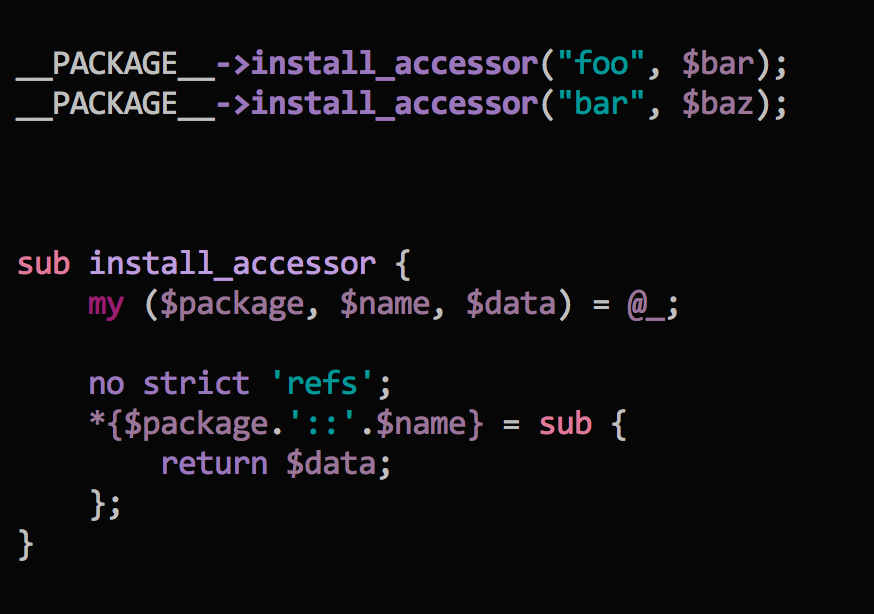
\includegraphics{cv-perl.png}
}
\end{figure}
\end{frame}

\begin{frame}{Real magic}
%accessors as an example of additional data attached to XS
%point to XSANY.any_ptr unsafety
%CV* cv = newXS_flags(full_name_buf, CAIXS_inherited_accessor, __FILE__, NULL, 0);
%sv_magicext((SV*)cv, (SV*)keys_av, PERL_MAGIC_ext, &sv_payload_marker, NULL, 0);
%SvREFCNT_dec_NN((SV*)keys_av);
%note difference from previous magic installeri

\begin{figure}
\scalebox{0.59}{
    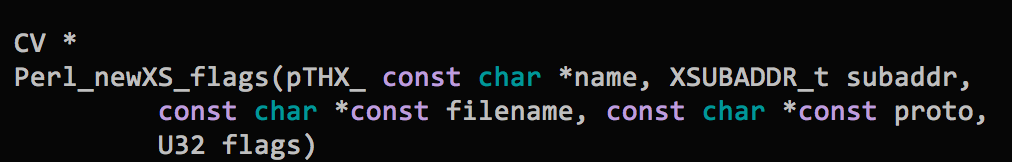
\includegraphics{cv-def.png}
}
\end{figure}

\pause


\begin{figure}
\scalebox{0.45}{
    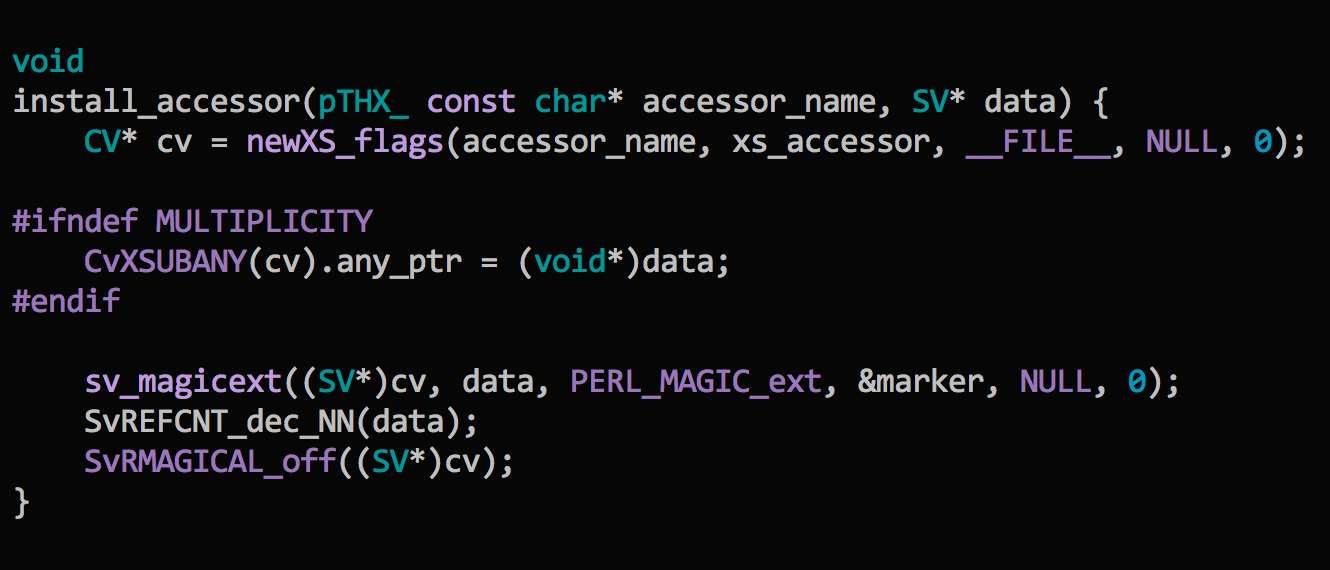
\includegraphics{cv-install.png}
}
\end{figure}
\end{frame}

\begin{frame}{}
\center{
    Questions?\\
    \vspace{2ex}
    github://\href{https://github.com/vovkasm/Class-Accessor-Inherited-XS}{Class::Accessor::Inherited::XS}\\
    \vspace{2ex}
    cpan://\href{http://search.cpan.org/~syber/Panda-XS/lib/Panda/XS.pm}{Panda::XS}
}
\end{frame}

\end{document}

